\documentclass[]{article}

\usepackage[T1]{fontenc}
\usepackage{graphicx}
\usepackage[colorlinks=true,allcolors=blue]{hyperref}
\usepackage[numbers]{natbib}

%\setlength{\parindent}{0pt} %to avoid the first line indent throughout the documen

\title{Variant calling from RNA-seq data using the GATK joint genotyping workflow}
\author{Jean-Simon Brouard}

\begin{document}

\maketitle

\begin{abstract}
Put the abstract here.
\end{abstract}

\section{Introduction}
Since the introduction of RNAseq, many researchers have seen the opportunity to use this data not only to quantify gene expression levels, but also for discover genomic variations \cite{Piskol2013}. Examples of such researches include a, b, c and d. Whereas trusted bioinformatic protocols exist for detecting sequence variants on a variety of DNAseq samples (germline DNA, whole-exome sequencing etc.) that come from distinct contexts \cite{Koboldt2020}, protocols designed to handle RNAseq data are scarce \cite{Piskol2013}. Among all resources available, many rely on the Genome Analysis Toolkit (GATK), an industry standard for variant discovery from next-generation sequencing (NGS) data, developped and maintainded by the Broad Institute.


At present the gold-standard for variant calling on RNAseq data is the GATK Per-sample workflow although an updated documentation for calling variants in RNAseq data is in the roadmap of the GATK experts \cite{GATK_best_RNAseq}. Currently, researchers interested in performing GATK variant calling on RNAseq data have the option of using the fully validated Per-sample workflow \cite{GATK_RNAseq_variant_discovery} or using an in-progress advanced workflow designed for cloud computing \cite{GATK_gatk4_rnaseq_github}. The Per-sample approach has several drawbacks, notably that only variable positions are reported and that the HaplotypeCaller engine cannot leverage population-wide information when calling variants \cite{Brouard2019, GATK_RNAseq_variant_discovery}.

An appealing alternative would be to use guidelines from the GATK Best practices relative to RNAseq data and to take advantage of joint genotyping approach which is avalaible for germline short variants and indels (ref). The joint-genotyping method has proven to be more sensitive, more flexible and to reduce computational challenges relative to the traditional calling approach \cite{GATK_jointCalling_1}. In addition, the latter approach has the advantage to facilitate the incremental discovery of variants that origin from distinct cohorts of samples. Technically, this can be achieved by combining parts of the GATK RNAseq workflow and parts of the GATK joint genotyping workflow.



In spite that the protocol described here largely use workflows and concepts developped by the GATK team, it should be pointed out that calling variants on RNAseq data with the joint genotyping workflow has still not been validated by GATK experts. We have shown previously this approach yield similar if not better results when compared to a Per-sample method \cite{Brouard2019}, but one would be advised to carefully examine the data to detect potential problems. Here we present a fully updated version of this approach in the form of an end-to-end analysis of RNAseq samples isolated from 50 cows for studying resistance to bovine paratuberculosis in dairy cattle.


As shown in figure 1, the workflow presented here involve several steps. In the data cleanup part, the raw RNAseq reads are prepared for RNAseq analysis according to the GATK Best practices relative to RNAseq data. In the variant discovery part, the analyis-ready RNAseq reads follow the germline Joint genotyping workflow up to the variant filtering steps.  

 
\begin{figure}
	\begin{center}
		
		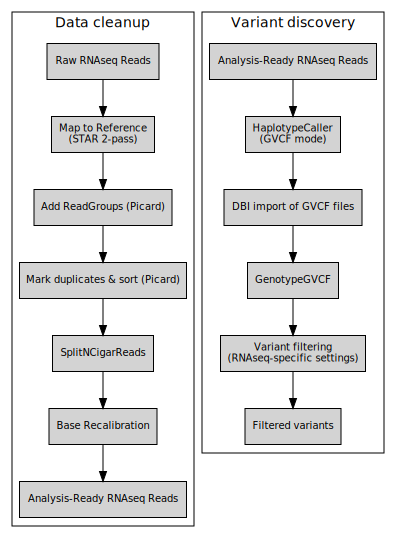
\includegraphics[width=0.7\textwidth]{misc/workflow.png}
		\caption[caption] {Workflow for calling variants from RNA-seq data using the GATK joint genotyping approach.}
		
	\end{center}
\end{figure}



In the next section, we describe how the diverse programs required to perform the whole analysis can be installed.

\section{Materials}

\subsection{Environment}


The vast majority of commands in this tutorial have been carefully tested and fully executed on a remote linux server working with the Sun Grid Engine (SGE) workload manager. Obviously, batch scripts will need to be slightly adapted if another workload manager is in place on your computer cluster or if you intend to perform the analysis locally on a linux machine.





\subsection{Installing bioinformatic programs}

\subsubsection{The GATK suite}

It is suggested to install the gatk4 suite in a separate conda environment. Assuming that you are familiar with the conda package management system, you could install all GATK programs in a environment called 'gatk4' with the following command:

\begin{verbatim}
conda create -n gatk4 -c bioconda gatk4 
\end{verbatim}




\subsubsection{The SRA toolkit programs}

You can easily download public sequences from the NCBI Sequence Read Archive (SRA) using the NCBI SRA toolkit. Detailed instructions about this tool can be found at \href{https://trace.ncbi.nlm.nih.gov/Traces/sra/sra.cgi?view=toolkit_doc}{https://trace.ncbi.nlm.nih.gov/Traces/sra/sra.cgi?view=toolkit\_doc.}. However, before using it, do not forget to configure the SRA toolkit program ( \href{https://github.com/ncbi/sra-tools/wiki/03.-Quick-Toolkit-Configuration}{https://github.com/ncbi/sra-tools/wiki/03.-Quick-Toolkit-Configuration}.


Once installed, export the SRA toolkit programs in you PATH:

\begin{verbatim}
export PATH=$PATH:$PWD/sratoolkit.2.10.9-ubuntu64/bin
\end{verbatim}

You can make this change persistent, by adding the previous line to your .bashrc file.


\subsubsection{The STAR aligner}

The best practices from GATK recommand to align RNA-seq reads with STAR (ref). 

Although you can retrieve and install the STAR aligner with conda, it can be installed easily by just downloading the latest STAR source from releases:

\begin{verbatim} 
wget https://github.com/alexdobin/STAR/archive/2.7.7a.zip
unzip 2.7.7a.zip
cd STAR-2.7.7a/
\end{verbatim}

You can then safely use the pre-compiled STAR executables located in the bin/ subdirectory. It is convenient to add the executables to your PATH:

\begin{verbatim}
export PATH=$PATH:$PWD/bin/Linux_x86_64
\end{verbatim}



\subsubsection{The Picard tools}

We will use the Picard tools to mark duplicated reads. One could find more information about the picard tools at: 
\href{https://broadinstitute.github.io/picard/}{https://broadinstitute.github.io/picard/.} One can download the pre-build java program with:

\begin{verbatim}
wget https://github.com/broadinstitute/picard/releases/download/2.25.0/picard.jar
\end{verbatim}

It is recommend to set up an environment variable to act as a shortcut. To make it persistent, simply, add a line to your .bashrc file:

\begin{verbatim}
export PICARD=/home/AAFC-AAC/brouardjs/bioinfo_programs/picard.jar
\end{verbatim}

Then, you would be able to call Picard tools with:

\begin{verbatim}
java -jar $PICARD
\end{verbatim}


\subsubsection{Samtools, BCFtools and HTSlib}
The Samtools, the BCFtools and the HTSlib are now divided in three separated repositories and can be found at \href{http://www.htslib.org/}{http://www.htslib.org/}{http://www.htslib.org/.

Mention the 2 2021 references that can be found on the htslib/documentation.

The Samtools are the gold-standard programs to read, write, edit, index and view alignments files in the SAM, BAM and CRAM format. In the same way, the BCFtools are the best option to manipulate sequence variants stored in the BCF2, VCF and gVCF format. The HTSlib are a C library designed to read and write high-throughput sequencing data that is used by both the Samtools and the BCFtools. Additionnaly, the HTSlib contains the tabix and bgzip utilities that are mandatory to work with vcf files.

The most straightforward way to make use of these three distinct packages is to build them independently. 

Use the commands below to install the Samtools:

\begin{verbatim}
wget https://github.com/samtools/samtools/releases/download/1.11/samtools-1.11.tar.bz2
bzip2 -d samtools-1.11.tar.bz2	
tar -xvf samtools-1.11.tar
cd  samtools-1.11
./configure --prefix=$HOME/bioinfo_programs/bcftools-1.12
\end{verbatim}

And you may wish to add the \\bin directory to your \$PATH:


\begin{verbatim}
export PATH=$PATH=/home/AAFC-AAC/brouardjs/bioinfo_programs/bcftools-1.12/bin
\end{verbatim}

The BCFtools and HTSlib can be installed with analogous commands.













\section{Methods}

\subsection{Downloading scripts used in this tutorial}

To reproduce the workflow presented here, a good starting point would be to download the following GitHub repository:

\begin{verbatim}
git clone https://github.com/soda460/RNAseq_GATK_JGW.git
\end{verbatim}

It contains all scripts described in this section as well as several text files that allow to easily reproduce the analysis presented here. Note that some scripts use relative paths. Therefore using the files/folder organization presentend in figure 2 will help to reproduce the results presented here with minimal changes.

\begin{figure}
\begin{center}

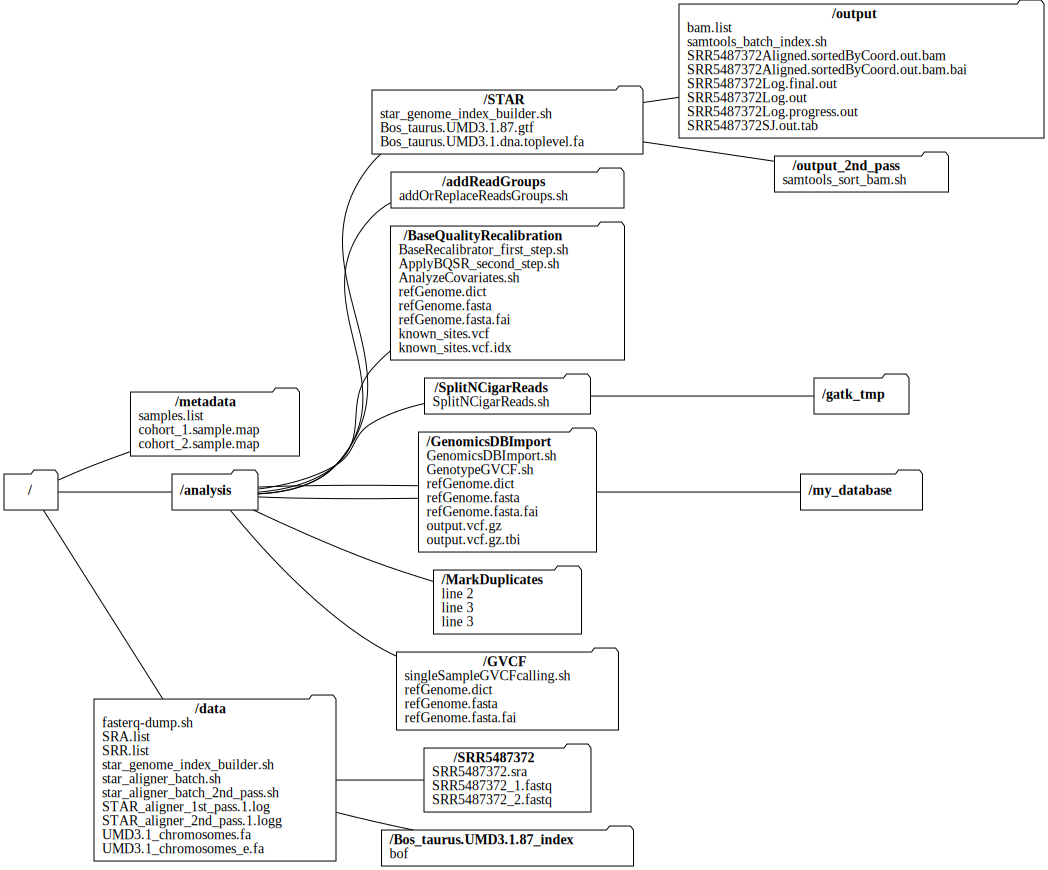
\includegraphics[width=1\textwidth]{misc/tree.png}
\caption[caption] {long desc.}

\end{center}
\end{figure}





\subsection{Downloading the MAP dataset from Sequence Read Archive}

We will use the complete RNA-seq raw sequences from \citep{Ariel2021}. However, rather than using the 72 samples presented in the article, we will use a subset of 24 representative samples of this study. The \textbf{SRA.list} file located in the data folder contains the SRA identifiers of these 24 samples:

\begin{verbatim}
SRS2153774
SRS2153779
SRS2153781
...
SRS2153841
SRS2153845
\end{verbatim}


To download these sequences (X Gb), navigate to the /data directory and download the 24 samples with the prefetch command from the SRAtoolkit:

\begin{verbatim}
prefetch --option-file SRA.list
\end{verbatim}

To extract fastq files from .sra files, the fasterq-dump command is required. For example, the following command will produce SRR5487396\_R1.fastq.gz and SRR5487396\_R2.fastq.gz files from the SRR5487396.sra archive.

\begin{verbatim}
fasterq-dump --split-files SRR5487396/SRR5487396.sra
\end{verbatim}

In practice, you will want to extract all downloaded sequence read archives, which are nested in distinct folders. Navigate to the /data folder and use the following qsub command to lauch the faster-qdump commands sequentially:

\begin{verbatim}
qsub -V -S /bin/bash -cwd -j y -pe smp 12 faster-qdump_sequential.sh
\end{verbatim}

where faster-qdump\_sequential.sh is a bash script containing instructions for the SGE workload manager and the code to iterate on all downloaded sequence read archives and produce the forward and reverse fastq files.

\begin{verbatim}
#! /bin/bash
#$ -N 'fasterq-dump'
#$ -o ./faster-qdump_log.txt
	
for i in `ls -d SRR*`; do
	cd $i
	fasterq-dump --split-files $i.sra
	cd ..
done
\end{verbatim}



However, executing the latter script would take a lot of times. To take advantage of the capacity of the cluster, one should may consider launching array tasks (task in parallel). To learn more about this, one can visit this page (SGE).

Before using the faster-qdump\_parallel.sh, we need to create a simple list file of the 24 SRR* folders present in the /data folder:

\begin{verbatim}
ls -d1 SRR5487???>SRR.list
\end{verbatim}

Be sure that the SRR.list file contains the 24 SRR identifiers (without the .sra extension) on separates lines before lauching the parallel version of fasterq.dump.sh with:
\begin{verbatim}
qsub -V -S /bin/bash -cwd -j y -t 1-24 -pe smp 4 faster-qdump_parallel.sh
\end{verbatim}

\noindent faster-qdump\_parallel.sh:
\begin{verbatim}
#!/bin/bash
#$ -N fasterq-dump
#$ -o ./fasterq-dump.$TASK_ID.log

input=$(head -n $SGE_TASK_ID SRR.list | tail -n 1)

cd $input
fasterq-dump --split-files $input.sra
cd ..
\end{verbatim}


Figure x show how a computationnaly intense task, namely the decompressing of an .sra archive, can be run at the same time with similar input files. This can be done by using the SGE task array capabilities. Technically, the same script is run multiple times, with different values taken by the single environment variable \$SGE\_TASK\_ID. Since many bioinformatic tasks used in this tutorial are computationally intensive, most of the scripts presented thereafter will be base on this model.


 

\subsection{Performing STAR alignment}

\subsubsection{Generating genome indexes files}

STAR genomes are available for a limited number of genomes on the Gingeras lab. We will use the for \textit{Bos taurus}  UMD3.1.87 annotations file since the UMD 3.1.1/bosTau8 version of the genome was used in \cite{Ariel2021}. The GTF file describes all exons whereas the .dna.toplevel.fa fasta file contains the corresponding sequences.



\begin{verbatim}
wget http://labshare.cshl.edu/shares/gingeraslab/www-data/dobin/\
STAR/STARgenomes/Old/ENSEMBL/bos_taurus/Bos_taurus.UMD3.1.87.gtf;

wget http://labshare.cshl.edu/shares/gingeraslab/www-data/dobin/\
STAR/STARgenomes/Old/ENSEMBL/bos_taurus/Bos_taurus.UMD3.1.dna.toplevel.fa;
\end{verbatim}

To prepare genome index files for STAR, use the genomeGenerate built-in STAR command.
Note that you have to create a directory where STAR could buid the index:

\begin{verbatim}
mkdir Bos_taurus.UMD3.1.87_index
\end{verbatim}

Then, build the index with:

\begin{verbatim}
qsub -V -S /bin/bash -cwd -j y -pe smp 6 star_genome_index_builder.sh
\end{verbatim}


\noindent star\_genome\_index\_builder.sh:
\begin{verbatim}
#! /bin/bash
#$ -N 'STAR_genome_builder'
#$ -o ./star_genome_builder_log.txt

STAR --runThreadN 6 \
--runMode genomeGenerate \
--genomeDir Bos_taurus.UMD3.1.87_index \
--genomeFastaFiles ./Bos_taurus.UMD3.1.dna.toplevel.fa \
--sjdbGTFfile ./Bos_taurus.UMD3.1.87.gtf \
--sjdbOverhang 99
\end{verbatim}



\subsubsection{Aligment with the STAR aligner}

At this step, we align our raw .fastq files with the STAR aligner.

\begin{verbatim}
qsub -V -S /bin/bash -cwd -j y -t 1-24 -pe smp 4 star_aligner.sh
\end{verbatim}


\noindent star\_aligner.sh:
\begin{verbatim}
#!/bin/bash
#$ -N 'STAR_aligner'
#$ -o STAR_aligner_1st_pass.$TASK_ID.log

input=$(head -n $SGE_TASK_ID SRR.list | tail -n 1)

mkdir -p ../analysis/STAR/output/$input

STAR --genomeDir ./Bos_taurus.UMD3.1.87_index \
--runThreadN 12 \
--readFilesIn  ./$input/$input"_1.fastq" ./$input/$input"_2.fastq" \
--outFileNamePrefix ../analysis/STAR/output/$input \
--outSAMtype BAM SortedByCoordinate \
--outSAMunmapped Within \
--outSAMattributes Standard
\end{verbatim}



\subsubsection{Adding Splice junctions (2nd mapping pass)}

GATK workflow recommend to perform 2-pass mapping with the STAR aligner. The 2nd mapping pass is identical to the first alignment except that all splice junctions discovered in the first pass are given as input to the programs, allowing to detect more reads mapping to novel junctions  \cite{Dobin2013}. Simply specify a list of all splice junctions files after the --sjdbFileChrStartEnd argument.


\begin{verbatim}
qsub -V -S /bin/bash -cwd -j y -t 1-24 -pe smp 4 star_aligner_2nd_pass.sh
\end{verbatim}

\noindent star\_aligner\_2nd\_pass.sh listing
\begin{verbatim}
#!/bin/bash
#$ -N 'STAR_aligner_2nd_pass'
#$ -o STAR_aligner_2nd_pass.$TASK_ID.log

input=$(head -n $SGE_TASK_ID SRR.list | tail -n 1)

mkdir -p ../analysis/STAR/output_2nd_pass/$input

STAR --genomeDir ./Bos_taurus.UMD3.1.87_index \
--runThreadN 4 \
--readFilesIn  ./$input/$input"_1.fastq" ./$input/$input"_2.fastq" \
--outFileNamePrefix ../analysis/STAR/output_2nd_pass/$input \
--outSAMtype BAM SortedByCoordinate \
--outSAMunmapped Within \
--outSAMattributes Standard \
--outTmpDir ../analysis/STAR/output_2nd_pass/_STARtmp_$SGE_TASK_ID \
--sjdbFileChrStartEnd \
../analysis/STAR/output/SRR5487372SJ.out.tab \
../analysis/STAR/output/SRR5487384SJ.out.tab \
...
../analysis/STAR/output/SRR5487430SJ.out.tab \
../analysis/STAR/output/SRR5487442SJ.out.tab
\end{verbatim}



\subsubsection{Sorting alignment files}


After you align your sequences. You will want that your .bam files to be indexed and sorted by coordinates. As mentioned earlier, STAR allows the output to be sorted by coordinates. If you have carefully followed this tutorial, there is no need to sort again your bam files and you can safely ignore the next step and jump to the next subheading. However, if for any reasons, your aligmnents files are not sorted adequately, the sorting by coordinates with the Samtools is as easy as :

\begin{verbatim}
samtools sort file.bam -o file_sorted.bam
\end{verbatim}

In a folder containing unsorted alignments, first prepare a list of bam files to be sorted with:

\begin{verbatim}
ls -1 *.bam > bam.list
\end{verbatim}

For our data, a qsub script would allow to re-sort our alignments files:


\begin{verbatim}
qsub -V -S /bin/bash -cwd -j y -t 1-24 -pe smp 2 samtools_sort_bam.sh
\end{verbatim}

This listing could also be used as a template to perform a variety of Samtools subcommands that involve renaming the output files.

\noindent samtools\_sort\_bam.sh
\begin{verbatim}
#!/bin/bash
#$ -V
#$ -N samtools_sort
#$ -o samtools_sort.$TASK_ID.log

input=$(head -n $SGE_TASK_ID bam.list | tail -n 1 | xargs basename -s '.bam')

samtools sort $input.bam -o $input"_sorted.bam"

\end{verbatim}


\subsubsection{Indexing alignment files}

BAM files (the binary analog of Sequence Alignment Mapping (SAM) files) are very efficient bioinformatic files designed to store high-throughput alignment data. Typically, they contain the result of the alignment of millions of sequencing reads against a reference genome and greatly benefit from being indexed by genomic positions for faster random access to the aligned reads at a specific locus. In practice most programs will not run in the absence of index files. Obviously, BAM files need to be sorted before being indexed. To index all bam files present in the STAR output\_2nd\_pass folder, first prepare a list of bam files to be indexed with:

\begin{verbatim}
ls -1 *.bam > bam.list
\end{verbatim}

Then, you can index all alignements in parallel with:

\begin{verbatim}
qsub -V -S /bin/bash -cwd -j y -t 1-24 -pe smp 2 samtools_batch_index.sh
\end{verbatim}

\noindent samtools\_batch\_index.sh

\begin{verbatim}
#!/bin/bash
#$ -N samtools_index
#$ -o samtools_index.$TASK_ID.log

input=$(head -n $SGE_TASK_ID bam.list | tail -n 1)

samtools index $input
\end{verbatim}





\subsection{Adding Read groups}

Contrarily to FASTQ files, SAM files have the capacity to handle large amount of metadata. A good practice would be to include informations about the reference genome and the samples in aligment files. Informations about the processing steps could also be stored in alignment files. Many programs, such as GATK, will add this metadata information when manipulating SAM/BAM files.


Most GATK commands involving BAM files require that Read groups have been defined. This step ensure that relevant informations about the sequencing process are assigned to each read in an alignment file. When this step is done carefully, it allow to mitigate the consequences of the sequencing biais that might arise due to how the sequencing process was performed \cite{GATK_ReadGroups}. For example, when samples are multiplexed, it is important to known which reads origin from the same library, which were sequenced on the same flowcell, etc. The GATK engine requires the presence of several read group fields to run without errors. To learn more about the Read groups as understand by the GATK team and to learn how to derive this information from read names, one should consult this page: \href{https://gatk.broadinstitute.org/hc/en-us/articles/360035890671-Read-groups}{https://gatk.broadinstitute.org/hc/en-us/articles/360035890671-Read-groups}.

Here, we will set the flowcells, sequencing lanes and sample barcode in the PU (Platform Unit) tag. We will also set the PL (Platform/technology used to produce the read) and LB (DNA preparation library identifier) tags. Note that the ID (Read group identifier) tag is overrided by the PU tag for base recalibration when it is defined.

Before running the main script, we will extract the first and fifth columns from our metadata file and place them in separate files, namely RGLB.txt and  RGPU.txt, that will be further used to populate the LB and PU read groups fields:

\begin{verbatim}
# Corresponding to the sample name
cut -f 1 -d ',' ../../metadata/metadata.txt | tail -n +2 > RGLB.txt

# Corresponding to the PU tag FLOW CELL 
cut -f 5 -d ',' ../../metadata/metadata.txt | tail -n +2 > RGPU.txt
\end{verbatim}

where /metadata/metadata.txt looks like:

\begin{verbatim}
sample,cowID,SRAID,Run,RGPU
A_CTL24,cowA,SRS2153774,SRR5487372,C5NL3ACXX.1.CAGATC
A_MAP24,cowA,SRS2153779,SRR5487376,C5NL3ACXX.1.TGACCA
B_CTL24,cowB,SRS2153781,SRR5487378,C5NL3ACXX.3.TGACCA
B_MAP24,cowB,SRS2153786,SRR5487382,C5NL3ACXX.3.GTGAAA
C_CTL24,cowC,SRS2153787,SRR5487384,C5K8FACXX.3.AGTCAA
C_MAP24,cowC,SRS2153791,SRR5487388,C5K8FACXX.3.GTCCGC
D_CTL24,cowD,SRS2153793,SRR5487390,C5K8FACXX.1.TGACCA
...
K_CTL24,cowK,SRS2153835,SRR5487432,C547FACXX.5.AGTCAA
K_MAP24,cowK,SRS2153839,SRR5487436,C547FACXX.5.GTCCGC
L_CTL24,cowL,SRS2153841,SRR5487438,C547FACXX.7.AGTCAA
L_MAP24,cowL,SRS2153845,SRR5487442,C547FACXX.7.GTCCGC
\end{verbatim}


The RGLB.txt file will therefore hold the library name for each 24 samples (e.g. C\_MAP24, which design a RNAseq library done on the cow C 24h post-infection with the MAP pathogen). The RGPU.txt hold the Platform Unit tag, which is made of three types of informations: the flowcell, the sequencing lane and the barcode identifiers, with the following format: {FLOWCELL\_BARCODE}.{LANE}.{SAMPLE\_BARCODE}. 


Use the following command to add read groups in alignments files:

\begin{verbatim}
qsub -V -S /bin/bash -cwd -j y -t 1-24 -pe smp 1 AddOrReplaceReadGroups.sh
\end{verbatim}

Since Bash arrays are zero-indexed, we use the value given by \$SGE\_TASK\_ID -1 to fetch the correct values in RGLB and RGPU arrays:

\noindent AddOrReplaceReadGroups.sh:
\begin{verbatim}
#!/bin/bash
#$ -N AddOrReplaceReadGroups
#$ -o logfile.$TASK_ID.log

eval "$(conda shell.bash hook)"
conda activate gatk4

SAMPLES="$HOME/jsb/springer2/RNAseq_GATK_JGW/metadata/samples.list"
BAMPATH="$HOME/jsb/springer2/RNAseq_GATK_JGW/analysis/STAR/output_2nd_pass"
OUTPUT="$HOME/jsb/springer2/RNAseq_GATK_JGW/analysis/addReadGroups"

readarray -t RGLB < ./RGLB.txt
readarray -t RGPU < ./RGPU.txt

input=$(head -n $SGE_TASK_ID $SAMPLES | tail -n 1)

java -jar $PICARD AddOrReplaceReadGroups \
I=$BAMPATH/$input"Aligned.sortedByCoord.out.bam" \
O=$OUTPUT/$input".bam" \
RGLB=${RGLB[$SGE_TASK_ID -1]} \
RGPL=ILLUMINA \
RGPU=${RGPU[$SGE_TASK_ID -1]} \
RGID=${RGPU[$SGE_TASK_ID -1]} \
RGSM=$input

conda deactivate
\end{verbatim}


When present, read groups are written in the header of BAM files. Thus, this simple UNIX trick allows one to quickly inspect the read groups associated to a BAM file:

\begin{verbatim}
samtools view -H sample.bam | grep '@RG'	
\end{verbatim}

After completion, we can iterate on all our .bam files and ensure that the reads groups have been correctly set:

\begin{verbatim}
for i in `ls *.bam | xargs basename -s '.bam'`;\
do echo $i; samtools view -H $i.bam | grep '@RG'; done
\end{verbatim}

\begin{verbatim}
SRR5487372
@RG	ID:C5NL3ACXX.1.CAGATC	LB:A_CTL24	PL:ILLUMINA	SM:SRR5487372	PU:C5NL3ACXX.1.CAGATC
SRR5487376
@RG	ID:C5NL3ACXX.1.TGACCA	LB:A_MAP24	PL:ILLUMINA	SM:SRR5487376	PU:C5NL3ACXX.1.TGACCA
SRR5487378
@RG	ID:C5NL3ACXX.3.TGACCA	LB:B_CTL24	PL:ILLUMINA	SM:SRR5487378	PU:C5NL3ACXX.3.TGACCA
SRR5487382
@RG	ID:C5NL3ACXX.3.GTGAAA	LB:B_MAP24	PL:ILLUMINA	SM:SRR5487382	PU:C5NL3ACXX.3.GTGAAA
\end{verbatim}





\subsection{MarkDuplicates}


Duplicate reads can arise from PCR duplication artifacts that take place during the library construction or from reading errors that occur during the sequencing process (optical duplicates). Regardless of their origin, these reads need to be identified in alignment files. The MarkDuplicate program from the Picard tools have many options to deal with these issue and output some metrics. For example, the program offer the possibility to completely remove the duplicate reads and to make the distinction between optical and PCR duplicates.

Here we will simply identified the duplicate reads in our .bam files before proceeding to the next step:

\begin{verbatim}
qsub -V -S /bin/bash -cwd -j y -t 1-24 -pe smp 2 MarkDuplicates.sh
\end{verbatim}


\noindent MarkDuplicates.sh:
\begin{verbatim}
#!/bin/bash
#$ -N MarkDuplicates
#$ -o logfile.$TASK_ID.log

SAMPLES="$HOME/jsb/springer/metadata/samples.list"
BAMPATH="$HOME/jsb/springer/analysis/addReadGroups"
OUTPUT="$HOME/jsb/springer/analysis/MarkDuplicates"

input=$(head -n $SGE_TASK_ID $SAMPLES | tail -n 1)

java -jar $PICARD MarkDuplicates \
I=$BAMPATH/$input".bam" \
O=$OUTPUT/$input"_marked_duplicates.bam" \
M=$OUTPUT/$input"_marked_dup_metrics.txt"
\end{verbatim}

\subsection{SplitNCigarReads}

Along with the non-GATK alignment of RNAseq raw sequences, the SplitNCigarReads step, (formerly called SplitNTrim step in previous versions of GATK workflows), is highly specific to RNAseq analysis. During this step reads that span splice junctions (for example reads that align over distinct exons) are split in smaller reads during the process. This step will produce alignments files that will adequately represent reads that span splice junctions. However, before doing this step, we need to get and prepare reference genome files.


\subsubsection{Preparing reference genome files}

Until now, we have work with STAR reference genome which barely contains sequences that are transcribed in RNA. In contrast, the GATK SplitNCigarReads command requires to use a complete reference sequence. At this point, one should be advised to download the same version of the full refence genome that was used to prepare the STAR genome.

To get the UMD3.1 assembly, visit \href{https://bovinegenome.elsiklab.missouri.edu/}{https://bovinegenome.elsiklab.missouri.edu/} and download the UMD3.1\_chromosomes.fa.gz and Ensembl79\_UMD3.1\_genes.gff3.gz files.


It is crucial that entries in the reference genome match the corresponding ones in the STAR genome. If you inspect the fasta headers of the UMD3.1\_chromosomes.fa, you will notice that each fasta entry contains many fields (e.g. gnl , UMD3.1 Accession numbers):

\begin{verbatim}
grep ">" UMD3.1_chromosomes.fa
\end{verbatim}


\begin{verbatim}
>gnl|UMD3.1|GK000010.2 Chromosome 10 AC_000167.1
>gnl|UMD3.1|GK000011.2 Chromosome 11 AC_000168.1
>gnl|UMD3.1|GK000012.2 Chromosome 12 AC_000169.1
...
>gnl|UMD3.1|GJ060407.1 GPS_000344847.1 NW_003101152.1
>gnl|UMD3.1|GJ060408.1 GPS_000344848.1 NW_003101153.1
\end{verbatim}

In contrast, the chromosomes entries in the STAR genome are quite different:

\begin{verbatim}
cat Bos_taurus.UMD3.1.87_index/chrName.txt | head -n 34
\end{verbatim}


One could use the following commands to rename the chromosome identifiers found in the Bos taurus UMD3.1 genome to the plain chromosome numbers as what is seen in the STAR genome:

\begin{verbatim}
sed -r s'/^>.+Chromosome\s+(\S+)\s+.+/>\1/' UMD3.1_chromosomes.fa > temp1.fa
grep ">" temp1.fa | head -n 40
sed -r s'/^>gnl\|UMD3\.1\|(\S+)+\s+.+/>\1/' temp1.fa > temp2.fa
grep ">" temp2.fa | tail -n +30 | head -n 10
mv temp2.fa refGenome.fasta
rm temp1.fa
\end{verbatim}


Along with the reference genome, many GATK tools will need a dictionary file ending in .dict and an index file ending in .fai.\href{ https://gatk.broadinstitute.org/hc/en-us/articles/360035531652-FASTA-Reference-genome-format}{ https://gatk.broadinstitute.org/hc/en-us/articles/360035531652-FASTA-Reference-genome-format}). These files need to share the same basename as the reference genome. You can prepare the index with:

\begin{verbatim}
samtools faidx refGenome.fasta
\end{verbatim}

On the other hand, use the GATK CreateSequenceDictionary tool to create the required .dict file:

\begin{verbatim}
gatk CreateSequenceDictionary -R refGenome.fasta
\end{verbatim}




\subsubsection{Running SplitNCigarReads}

Having prepared reference genome files and index, we are ready to lauch the following SplitNCigarRead listing:


\begin{verbatim}
qsub -V -S /bin/bash -cwd -j y -t 1-24 -pe smp 4  SplitNCigarReads.sh
\end{verbatim}



\begin{verbatim}
#!/bin/bash
#$ -N SplitNCigarReads
#$ -o SplitNCigarReads.$TASK_ID.log
	
eval "$(conda shell.bash hook)"
conda activate gatk4
	
SAMPLES="$HOME/jsb/springer/metadata/samples.list"
BAMPATH="$HOME/jsb/springer/analysis/MarkDuplicates"
OUTPUT="$HOME/jsb/springer/analysis/SplitNCigarReads"
	
input=$(head -n $SGE_TASK_ID $SAMPLES | tail -n 1)

gatk SplitNCigarReads \
-R refGenome.fasta \
-I $BAMPATH/$input"_marked_duplicates.bam" \
-O $OUTPUT/$input"_SplitNCigarReads.bam" \
--tmp-dir $output/gatk_tmp
	
conda deactivate
\end{verbatim}



\subsection{Performing base quality score recalibration}

Base Quality Score Recalibration (BQSR) is an optional, but highly recommended step, that figure in DNAseq and RNAseq GATK best practices workflows. This complex procedure, which involves binning and machine learning consist of re-evaluating all base quality scores assigned by sequencing machines which are prone to systematic technical errors \cite{GATK_BaseQuality}. This procedure lead to more accurate base calls, a situation that improve the accuracy of variant calling overall. More details about how the model is build and how new quality scores are computed can be found at \href{https://gatk.broadinstitute.org/hc/en-us/articles/360035890531-Base-Quality-Score-Recalibration-BQSR-}{https://gatk.broadinstitute.org/hc/en-us/articles/360035890531-Base-Quality-Score-Recalibration-BQSR-}.

\subsubsection{Using BaseRecalibrator}

In the first key step  a model of covariation is build with two components: the alignement given as input (bam files) and a set of known variants (VCF file). The BaseRecalibrator will then produce a recalibration file which is used in the second key step of the procedure. To perform this task one would need a source of reliable variants in the investigated genome. With human data and other common model organisms, it would be easy to find such sources of variants thanks to the existence of variation databases. Here we use a single VCF file containing the results of the BovineSNP50 genotyping BeadChip to train the model, but you can feed the model with several VCF files.

%BaseRecalibrator first script
\begin{verbatim}
#!/bin/bash
#$ -V
#$ -N BaseRecalibrator
#$ -S /bin/bash
#$ -cwd
#$ -j y
#$ -b n
#$ -e e
#$ -o BaseQualityRecalibration_$TASK_ID.log
#$ -q all.q
#$ -t 1-24
#$ -pe smp 4

eval "$(conda shell.bash hook)"
conda activate gatk4

SAMPLES="$HOME/jsb/springer/metadata/samples.list"
BAMPATH="$HOME/jsb/springer/analysis/SplitNCigarReads"
OUTPUT="$HOME/jsb/springer/analysis/BaseQualityRecalibration"

input=$(head -n $SGE_TASK_ID $SAMPLES | tail -n 1)

gatk BaseRecalibrator \
-R ./refGenome.fasta \
-I $BAMPATH/$input"_SplitNCigarReads.bam" \
--known-sites ./jsb.vcf \
-O $OUTPUT/$input"_recal_data.table"

conda deactivate
\end{verbatim}





\subsubsection{Using ApplyBQSR to adjust the scores}

In the second step of the BaseQuality recalibration process, the GATK ApplyBQSR command assigns new scores to each base based on the model produced in the first step and produces new BAM files that reflet these changes.  


%ApplyBQSR listing
\begin{verbatim}
#!/bin/bash

#$ -V
#$ -N ApplyBQSR
#$ -S /bin/bash
#$ -cwd
#$ -j y
#$ -b n
#$ -e e
#$ -o ApplyBQSR_$TASK_ID.log
#$ -q all.q
#$ -t 1-24
#$ -pe smp 4

eval "$(conda shell.bash hook)"
conda activate gatk4

SAMPLES="$HOME/jsb/springer/metadata/samples.list"
BAMPATH="$HOME/jsb/springer/analysis/SplitNCigarReads"
OUTPUT="$HOME/jsb/springer/analysis/BaseQualityRecalibration"

echo $SAMPLES
input=$(head -n $SGE_TASK_ID $SAMPLES | tail -n 1)

gatk ApplyBQSR \
-R ./refGenome.fasta \
-I $BAMPATH/$input"_SplitNCigarReads.bam" \
--bqsr-recal-file $OUTPUT/$input"_recal_data.table" \
-O $OUTPUT/$input"_recal.bam"

conda deactivate
\end{verbatim}

\subsubsection{Comparing pre- and post-recalibration metrics}

To visualize the effect of the procedure, one can build a seconde model and generate plots with data before and after recalibration \cite{GATK_BaseQuality} The GATK command AnalyzeCovariates was created for that purpose as in the following example:

\begin{verbatim}
gatk AnalyzeCovariates \
-before recal1.table \
-after recal2.table \
-plots AnalyzeCovariates.pdf
\end{verbatim}



\subsection{Joint genotyping Variant Calling}


The Base recalibration being the final step in the Data cleanup part of the workflow present here (figure 1), we are ready for discovering variants from our analysis-ready RNAseq reads with the joint genoyping approach. Again, this procedure involves several steps which are part of the Germline short variant discovery (SNPs + Indels) Best Practices Workflows \cite{GATK_BP_Germline}. First, we will call variants per-sample with the HaplotypeCaller engine, then we will merge GVCF files with the GenomicsDBImport tool and finally we will perform joint genotyping with the GATK GenotypeGVCFs command.




\subsubsection{Calling variants per-sample (GVCF mode)}
%GCVF listing


In this step, the GATK variant calling engine, HaplotypeCaller, identifies potential variation sites and record them in GVCF files. This is why this step has been called "GVCF workflow". GVCF files act as intermediate between analysis ready reads (BAM files) and the final joint analysis of multiple samples \cite{GATK_jointCalling_1}. Such intermediate files facilitate the incremental discovery of variants and should be kept since they can be reused in novel rounds of joint genotyping analysis. Our listing to produce GVCF files for each sample reads as follow:


\begin{verbatim}
#!/bin/bash
#$ -V
#$ -N callingGVCF
#$ -S /bin/bash
#$ -cwd
#$ -j y
#$ -b n
#$ -e e
#$ -o singleSampleCallingGVCF_$TASK_ID.log
#$ -q all.q
#$ -t 1-24
#$ -pe smp 4

eval "$(conda shell.bash hook)"
conda activate gatk4

SAMPLES="$HOME/jsb/springer/metadata/samples.list"
BAMPATH="$HOME/jsb/springer/analysis/BaseQualityRecalibration"
OUTPUT="$HOME/jsb/springer/analysis/GVCF"

echo $SAMPLES
input=$(head -n $SGE_TASK_ID $SAMPLES | tail -n 1)

gatk --java-options "-Xmx4g" HaplotypeCaller \
-R ./refGenome.fasta \
-I $BAMPATH/$input"_recal.bam" \
-O $OUTPUT/$input".g.vcf.gz" \
-ERC GVCF

conda deactivate
\end{verbatim}





\subsubsection{Merging of GCVF files}

This step has been revised recently by GATK experts by the addition of the novel GATK GenomicsDBImport command. It resembles the former CombineGVCFs command, but promises better performances for parsing of VCF files and computing of values stored in the VCF INFO fields. More details can be found at \href{https://gatk.broadinstitute.org/hc/en-us/articles/360036883491-GenomicsDBImport}{https://gatk.broadinstitute.org/hc/en-us/articles/360036883491-GenomicsDBImport}. Interestingly, under the hood, this command make use of a novel data managament system called  TileDB which is particluarly useful for representing huge sparse 2D arrays such as the genomic data found in VCF files \cite{Papadopoulos2016}. 


The command requires a map files that list the full paths of all GVCF files to be included in the resulting database. 

The -L option specifies the range genomic intervals on which the command operate and may be used several times. Since, we are interested to call variants on all bovine autosomes, we used it many times in the following listing:


%GenomicsDBImport listing
\begin{verbatim}
eval "$(conda shell.bash hook)"
conda activate gatk4

SAMPLES="$HOME/jsb/springer/metadata"
OUTPUT="$HOME/jsb/springer/analysis/GenomicsDBImport"

gatk --java-options "-Xmx4g -Xms4g" \
GenomicsDBImport \
--genomicsdb-workspace-path $OUTPUT/"my_database" \
-L 1 \
-L 2 \
...
-L 28 \
-L 29 \
--sample-name-map $SAMPLES/"cohort_1.sample_map" \
--tmp-dir $HOME/jsb/tmp \
--reader-threads 5
conda deactivate

\end{verbatim}


\subsubsection{Joint genotyping}

The final step in this variant calling workflow, which is actually the joint genotyping step, is performed with the GATK GenotypeGVCFs command (  \href{https://gatk.broadinstitute.org/hc/en-us/articles/360037057852-GenotypeGVCFs}{https://gatk.broadinstitute.org/hc/en-us/articles/360037057852-GenotypeGVCFs}). During this operation, all samples for which variant have been pre-called with HaplotypeCaller are jointly genotyped. This step could be rerun when new samples are available, allowing the so-called incremental discovery of variants.


The command take as argument a GenomicsDB workspace created by GenomicsDBImport, which can be seen as a sophisticated database that facilitate the parsing of the genomic data present in GVCF files. Alternatively, a single multi-sample GCVF file produced by CombineGVCFs (used after HaplotypeCaller) can also be given as input.

%GenotypeGVCFs listing
\begin{verbatim}
#!/bin/bash
#$ -V
#$ -N GenotypeGVCF
#$ -S /bin/bash
#$ -cwd
#$ -j y
#$ -b n
#$ -e e
#$ -o GenotypeGVCF.log
#$ -q all.q
#$ -pe smp 4

eval "$(conda shell.bash hook)"
conda activate gatk4

gatk --java-options "-Xmx4g" GenotypeGVCFs \
-R refGenome.fasta \
-V gendb://my_database \
-O output.vcf.gz
conda deactivate
\end{verbatim}




\subsection{Querying variants}


As mentionned earlier, by design, BCFtools are optimized to query and manipulate VCF files. Therefore, it is worth the pain to familiarize with these tools rather than using the plain VCF files with UNIX tricks. In addition, since BCFtools work well with compressed files it would be a waste of time to compress or extract VCF files not to mention the risk of corrupting or erasing a VCF file. Because one can easily erase a file by mistakes when attempting to redirect the result of querying and filtering commands, it is a good practice to keep a copy of the primary VCF output file in a safe place.

That said, the BCFtools command are highly versatile and can be used in several circumstances ranging from performing simples queries to applying complex filters. Here a few examples:

To get a list of all samples present in a VCF files:

\begin{verbatim}
bcftools query -l output.vcf.gz
\end{verbatim}

To get useful metrics, like the sequencing depth or the ratio of transitions and transversions use the buil-in stats command:
\begin{verbatim}
bcftools stats output.vcf.gz  > stats.txt
\end{verbatim}

To quickly see the numbers of variants that fall in each category:
\begin{verbatim}
bcftools stats output.vcf.gz | grep -E "^SN"
\end{verbatim}

To mask the VCF header and see variants from selected samples in a specific regions:
\begin{verbatim}
bcftools view -H -s SRR5487378,SRR5487390 -r 1:1-100000 output.vcf.gz
\end{verbatim}


It is possible to extract fetch some columns and manipulate them with the query command for example:
\begin{verbatim}
bcftools query -i'QUAL>20 && INFO/DP>10' -f'chr%CHROM pos:%POS Q:%QUAL DP=%INFO/DP\n' output.vcf.gz | head -n 10
chr1 pos:242647 Q:2073.95 DP=46
chr1 pos:242649 Q:2073.95 DP=46
chr1 pos:245489 Q:31.59 DP=12
chr1 pos:246301 Q:75.98 DP=15
chr1 pos:246448 Q:190.97 DP=15
chr1 pos:247141 Q:151.58 DP=11
chr1 pos:247219 Q:66.88 DP=12
chr1 pos:247224 Q:66.88 DP=12
chr1 pos:247245 Q:98.22 DP=13
chr1 pos:248413 Q:67.87 DP=22

\end{verbatim}





\subsection{Filtering variants}


Filtering variants is an active aera of research and the reader is invite to consult the GATK Best practices workflows documentation to be aware of all the novelties.

One would be interested to firstly removed low quality calls with low read depth:

\begin{verbatim}
bcftools filter -e "QUAL >= 20.0 && INFO/DP >= 10" output.vcf.gz > filtered.vcf.gz
\end{verbatim}


Be aware that both INFO/DP and FORMAT/DP fields exist and have different meanings.


Contrarily to DNAseq workflows where sophisticated methods for filtering variants are available (VQSR and CNNScoreVariants), the current recommandation for RNAseq is to use hard filters as described in the canonical RNAseq Best practice RNAseq short variant discovery workflow \cite{GATK_RNAseq_variant_discovery}. The GATK and Picard tools has several commands to filter variants although the BCFtools filter and view commands could also be used. To perform hard filter, one could use the GATK VariantFiltration command  (\href{https://gatk.broadinstitute.org/hc/en-us/articles/360037269391-VariantFiltration}{https://gatk.broadinstitute.org/hc/en-us/articles/360037269391-VariantFiltration}) which is designed to filter variants on the basis of annotations in INFO or FORMAT VCF fields.

Naturally, the extend of filtration steps that could be done depends on the nature of the downstream analysis that will be performed. Among the numerous filtering that could be done, we present here a filtering step specific to RNAseq data that was proposed by GATK experts in previous Best practices workflows, but that should be still appropriate. It consist of filtering out clusters of at least 3 SNPs that are within a window of 35 bases between them.


\begin{verbatim}
gatk VariantFiltration \
-R refGenome.fasta \
-V output.vcf.gz \
-O filtered.vcf.gz \
--cluster-window-size 35 \
--cluster-size 3
\end{verbatim}

The GATK command write PASS or SnpCluster in the FILTER field (rather than the dot that was present in VCF file given as input) and add the following lines to the output VCF header:

\begin{verbatim}
##FILTER=<ID=SnpCluster,Description="SNPs found in clusters">
##FILTER=<ID=PASS,Description="All filters passed">
\end{verbatim}


Thus, to actually get rid off these variants, use the BCFtools view command with the --apply-filter option:
\begin{verbatim}
bcftools view --apply-filters .,PASS filtered.vcf.gz | bgzip -c > purged.vcf.gz
\end{verbatim}


Note how the BCFtools are fully integrated with other UNIX commands. Here the filtered VCF files is given to the HSTlib bgzip program that compress it before that the UNIX file redirection operator write the result to a new file. You can validate that SNP clusters do not appear in the purged.vcf.gz with:


\begin{verbatim}
bcftools view purged.vcf.gz | grep SnpCluster
\end{verbatim}

In DNA-seq, the generic current recommendation is to filter out variants based on Fisher Strand values (FS > 60.0) and Quality by depth values (QD < 2.0).

At first, we could be interested to know how many variants will be excluded with FS > 60.0:

\begin{verbatim}
bcftools filter -i 'FS > 60' purged.vcf.gz | bcftools view -H | wc -l
2610
\end{verbatim}

and how many variants will be excluded with QD < 2.0:

\begin{verbatim}
bcftools filter -i 'QD < 2.0' purged.vcf.gz | bcftools view -H | wc -l
15089
\end{verbatim}


To correctly translate the previous recommendation and combine the two criterions, one would be advised to use the logical '||' operator (OR) (rather than '\&\&' (AND) ) because one will want to throw out any variants with fail at least one criterion:

\begin{verbatim}
bcftools filter -i 'FS > 60 || QD < 2.0' purged.vcf.gz | bcftools view -H | wc -l
17273
\end{verbatim}


To actually remove these variants, simply use the -e option (--exclude) and create a new file:

\begin{verbatim}
bcftools filter -e 'FS > 60 || QD < 2.0' purged.vcf.gz | bgzip -c > newfile.vcf.gz
\end{verbatim}


A very intersting ressource to adequately applying other hard filters can be found at \href{https://gatk.broadinstitute.org/hc/en-us/articles/360035890471-Hard-filtering-germline-short-variants}{https://gatk.broadinstitute.org/hc/en-us/articles/360035890471-Hard-filtering-germline-short-variants}.




\subsection{Examining and visualizing alignment files}

At a moment you will want to visualize alignments files and see the correspondance between called variants found in VCF files and the final alignments.  

Tablet \href{https://ics.hutton.ac.uk/tablet/download-tablet/}{https://ics.hutton.ac.uk/tablet/download-tablet/} and the Integrated Genome viewver (ref) are good choices. 


To add track to use the gff3 file and again we would need to rename entries to macth those in our .bam files.



\subsubsection{The gff3 file}

With the command below, one can see the number of features annotated for each ID in the gff3 file: 

\begin{verbatim}{bash}
	cat Ensembl79_UMD3.1_genes.gff3 | cut -f 1 | uniq -cd
\end{verbatim}


%output of cat Ensembl79 gff3
Here a summary of the previous command:
\begin{verbatim}
	21287 GK000001.2
	18819 GK000030.2
	26235 GK000002.2
	29793 GK000003.2
	...
	14 GJ058430.1
	31 GJ058425.1
	...
	23 GJ059509.1
	3 GJ058729.1
	3 GJ060027.1
	3 GJ058256.1
\end{verbatim}

Therefore, to ensure that the gff3 chromosome IDs match those presennt in our alignment files, we need to slightly edit this file to replace the pattern used for the chromosome IDs (GK + 0000 + chromosome number) by solely the chromosome number. This could be done easily with sed:

\begin{verbatim}
	sed -r s'/^GK[0]+([0-9]+).2/\1/'g Ensembl79_UMD3.1_genes.gff3 \
	> Ensembl79_UMD3.1_genes_e.gff3
\end{verbatim}

Obvisouly it is good idea to inspect the edited file to ensure that the desired changes have been done properly.



\begin{verbatim}
	gunzip -c output.vcf.gz > output.vcf
\end{verbatim}


Here a screenshot of sample SRR5487372

\begin{figure}
\begin{center}

\includegraphics[width=1\textwidth]{misc/chr11_region.png}
\caption[caption] {Screenshot from the Tablet genome browser. Sample SRR5487372 is heterozygote for the rs43668743 SNP (chr11 pos:21401262) in an intergenic region of the \textit{SOS1} gene.}

\end{center}
\end{figure}






tabix -c purged.vcf.gz

bcftools view -s SRR5487372 -r 11:15063000-15068675  purged.vcf.gz

Figure 3 show an heterozygous call in a exonic region on chromosome 11.









\bibliographystyle{unsrtnat}
\bibliography{bibliography/RNAseq_VC}





\end{document}
